\documentclass{article}
\usepackage{amsmath}
\usepackage{setspace}
\usepackage{graphicx} % Add the graphicx package for including graphics
\usepackage{listings}
\lstset{
  language=Python,
  breaklines=true,
  basicstyle=\ttfamily,
  keywordstyle=\bfseries,
  frame=single
}


\renewcommand{\baselinestretch}{2} 

\begin{document}
    \begin{center}
    {\Large Homework 0}\\
    \end{center}

\section*{Exercise 1}
$\begin{bmatrix}
    0 & 0 \\
    0 & 0
\end{bmatrix}$
0 indipendent rows, so rank is 0.
\section*{Exercise 4}
$A=\begin{bmatrix}
    A_{11} & A_{12} & A_{13} \\
    A_{21} & A_{22} & A_{23} \\
    A_{31} & A_{32} & A_{33}
\end{bmatrix}\quad
B=\begin{bmatrix}
    B_{11} & B_{12} & B_{13} \\
    B_{21} & B_{22} & B_{23} \\
    B_{31} & B_{32} & B_{33}
\end{bmatrix}$
\\
$AB=\begin{bmatrix}
    A_{11}B_{11}+A_{12}B_{21}+A_{13}B_{31} & A_{11}B_{12}+A_{12}B_{22}+A_{13}B_{32} & A_{11}B_{13}+A_{12}B_{23}+A_{13}B_{33} \\
    A_{21}B_{11}+A_{22}B_{21}+A_{23}B_{31} & A_{21}B_{12}+A_{22}B_{22}+A_{23}B_{32} & A_{21}B_{13}+A_{22}B_{23}+A_{23}B_{33} \\
    A_{31}B_{11}+A_{32}B_{21}+A_{33}B_{31} & A_{31}B_{12}+A_{32}B_{22}+A_{33}B_{32} & A_{31}B_{13}+A_{32}B_{23}+A_{33}B_{33}
\end{bmatrix}$
\\
\\
$trAB=A_{11}B_{11}+A_{12}B_{21}+A_{13}B_{31}+A_{21}B_{12}+A_{22}B_{22}+A_{23}B_{32}+A_{31}B_{13}+A_{32}B_{23}+A_{33}B_{33}$
\\
$\frac{\partial trAB}{\partial A}=\begin{bmatrix}
    B_{11} & B_{21} & B_{31} \\
    B_{12} & B_{22} & B_{32} \\
    B_{13} & B_{23} & B_{33}
\end{bmatrix}=B^T$
\\
\section*{Exercise 13}
$p=p_0+\dot{p}t+\frac{1}{2}\ddot{p}t^2$
\subsection*{a}
$x = \begin{bmatrix}
    p_0 + \dot{p}t + \frac{1}{2}\ddot{p}t^2 \\
    \dot{p} + \ddot{p}t \\
    \ddot{p}
\end{bmatrix}$
\quad
$A=\begin{bmatrix}
    0 & 1 & 0 \\
    0 & 0 & 1 \\
    0 & 0 & 0
\end{bmatrix}$
\\
$\dot{x}=\begin{bmatrix}
    0 & 1 & 0 \\
    0 & 0 & 1 \\
    0 & 0 & 0
\end{bmatrix}x$
\subsection*{b}
$e^{At}=\sum_{j=0}^{\infty}\frac{At^{j}}{j!}=I+At+\frac{At^2}{2!}=
\begin{bmatrix}
    1 & 0 & 0 \\
    0 & 1 & 0 \\
    0 & 0 & 1
\end{bmatrix}+\begin{bmatrix}
    0 & 1 & 0 \\
    0 & 0 & 1 \\
    0 & 0 & 0
\end{bmatrix}t+\frac{1}{2}
\begin{bmatrix}
    0 & 0 & 1 \\
    0 & 0 & 0 \\
    0 & 0 & 0
\end{bmatrix}t^2 \\
= \begin{bmatrix}
    1 & t & \frac{1}{2}t^2 \\
    0 & 1 & t \\
    0 & 0 & 1
\end{bmatrix}$ 
\subsection*{Exercise 19}
\subsubsection*{a}
$x_1(t)=0 \quad x_2(t)=0$ \\
$0=\frac{Ku-gx_2}{x_3}-\frac{GM}{(R+x_1)^2}$\\
$0=\frac{Ku}{x_3}-\frac{GM}{R^2}\rightarrow x_3=\frac{KuR^2}{GM}$\\
Since $\dot{x}_3=-u \quad u(t)=e^{-\frac{GM}{kR^2}t}$
\subsubsection*{b}
$x_3=\frac{kR^2}{GM}e^{-\frac{GM}{kR^2}t}$
\subsubsection*{c}
$A=\begin{bmatrix}
    \frac{\partial{f}}{\partial x}
\end{bmatrix}
=\begin{bmatrix}
    0 & 1 & 0\\
    \frac{2GM}{(R+x_1)^3} & -\frac{g}{x_2} & -\frac{Ku-gx_2}{x_3^2}\\
    0 & 0 & 0
\end{bmatrix}\\
B=\begin{bmatrix}
    \frac{\partial{f}}{\partial u}
\end{bmatrix}
=\begin{bmatrix}
    0 \\
    \frac{K}{x_3} \\
    -1
\end{bmatrix}\\
\dot{x}=Ax+Bu$

\begin{lstlisting}
import numpy as np; from scipy.integrate import solve_ivp; import matplotlib.pyplot as plt

k, g, G, M, R, delta_u_list, t_span, y0 = 1000, 50, 6.673e-11, 5.98e24, 6.37e6, [10, 100, 300], [0,5], [0,0]
u, u_int = lambda t: np.exp(-G*M/(k*(R**2))*t), lambda t, delta_u: (G*M)/(k*(R**2))*u(t)*10000+np.abs(np.cos(t))*delta_u
non_linear_system = lambda t, y, delta_u: [y[1], -((k * u(t) - g * y[1]) / u_int(t, delta_u) - G * M / (R + y[0]) ** 2)]
linear_system = lambda t, y, delta_u: [y[1], -2*G*M*y[0]/(R**3)-g*y[1]/(u_int(t, delta_u))+(k*10000*u(t)/u_int(t, delta_u))-k*10000*u(t)/u_int(t, delta_u)]
solution = lambda delta_u, function: solve_ivp(function, t_span, y0, args=(delta_u,), t_eval=np.linspace(0, 5, 1000))
 
delta_u = 10
print(solution(delta_u, linear_system))
[plt.plot(np.linspace(0, 5, len(solution(delta_u, linear_system).y[0])), solution(delta_u, linear_system).y[0], '--', label=r'$\Delta u={}$'.format(delta_u)) for delta_u in delta_u_list]
[plt.plot(np.linspace(0, 5, len(solution(delta_u, non_linear_system).y[0])), solution(delta_u, non_linear_system).y[0], label=r'$\Delta u={}$'.format(delta_u)) for delta_u in delta_u_list]
plt.xlabel('Time'), plt.ylabel('Altitude'), plt.xlim(0, 5), plt.legend(), plt.savefig('Nonlinear System'), plt.show()
\end{lstlisting}
\begin{figure}
    \centering
    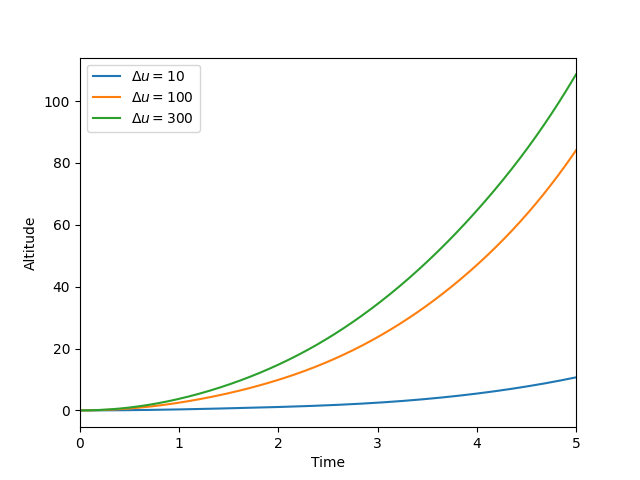
\includegraphics[width=0.8\textwidth]{Nonlinear System.png}
    \caption{Nonlinear System}
\end{figure}
\end{document}